% This file is based on the "sig-alternate.tex" V1.9 April 2009
% This file should be compiled with V2.4 of "sig-alternate.cls" April 2009

\documentclass{sig-alternate}

\usepackage{url}
\usepackage{color}
\usepackage{enumerate}
\usepackage{balance}
\permission{}
\CopyrightYear{2013}
%\crdata{0-00000-00-0/00/00}
\begin{document}

\title{Visualization of Music Artist Networks }
\numberofauthors{1}
\author{
\alignauthor
Anonymous
}

\maketitle

\begin {abstract}
Our project aims to create a visual network of music artists 
and their relations to other music artists. Data will be obtained 
from a large number of Wikipedia articles using techniques such 
as plain text analysis. An auxiliary database will be developed to 
create structure out of the semi-structured raw data we will receive. 
This will allow for an efficient searching and give way to a faster user interface. 
The user interface will be an application that will use an interactive network 
display that shows the following: the original queried artist, the 
connections that artist has to other artists, and the connections 
of other artists in turn. Visualization of our data is one of 
the main focuses of this project and will be facilitated by our
 interactive network display application, creating an enjoyable and relatively 
simple experience for the user to search our structured database.

\end{abstract}

\section{Overview}
\label{overview}
The goal of this project is to develop an application that will create 
a visual map of a music artist's social network. For example, say you query 
for ``Dr. Dre". The query will display how Dr. Dre is related to Eminem as 
his producer, and to N.W.A as a former member of the group. If you then 
choose ``N.W.A.", the application will explain that N.W.A. is also related to 
 Ice Cube and MC Ren because they are also former members. The goal is 
to ultimately have all of the relations to the original query, in this case Dr. Dre, 
displayed in an interactive graph that the user can use to jump from one 
artist, band, or fact, to another using the information mined from the data. 
Data visualization is the goal of our interactive map. Making it easy 
for the user to query artists and see all of their relations will 
be facilitated by our interactive graphical application. Also, the data domain 
of ``music'' is something almost everyone can relate to, making it 
a good choice for this project; many people can claim to have domain 
expertise in the category of music.

The dataset will be taken from a dump of the English Wikipedia. This implies 
that we will be mining semi-structured data from the wikicode that generates an 
article text. Also, many of the pages contain a subsection called ``Discography'' 
that will need to be mined for this project. To gather the rest of the data, 
plain text searches can be used to find ``produced by", ``collaborated with", 
or ``shared stage with'' relationships, just to name a few. After mining this 
semi-structured data, we will be able to store it as structured data in a database 
that our interactive graph can query. This will be more efficient than the 
application querying the raw data. 


\section{Dataset}
\label{dataset}

The first step in creating our database was the collection of the raw data.
In order to do this, a database ``artistgraph'' was created and a table creation
script was run matching the structure of a wikipedia database. Next, a XML dump from the Wikipedia was downloaded and
mwdumper 1.16, a Java application, was used to extract the data from the XML and load it
into our ``artistgraph'' database. The application contained a graphical user interface
or ``GUI'' which caused some errors. To avoid manipulating the code to resolve these errors,
the command line method of mwdumper was preferred. However, after 246,000 records, the 
Java program would produce an error due to the maximum allowed packet settings in MySQL
being too low. This value is small by default in order to catch large, incorrect packets.
This was updated from 16MB to 123MB, resolving the issue.

After running the program
for more than 24 hours, less than 2 million records were loaded. This prompted an 
investigation into why it was loading so slowly. The issue was that the main tables 
(page, revision, and text) have auto increment keys and indices, which were incremented after each insert.
Because of this, the insert rate was about 13 records per second, which, for
millions of records, is unacceptably slow. To resolve this issue, the tables
were truncated, and the auto increment definition was removed. The indices
of the tables were also removed along with the assignment of primary keys. The altered
script was executed to recreate the tables, and the Java program was run. This resulted
in a loading speed between 600 and 900 records per second. 

This code ran until just shy of 9 million records were loaded. At this point, an unknown error occurred.
Because it is believed that 9 million records is a large majority of the
database, the Java code and the XML file have not been examined yet, since the project is still in an early stage of development. 
With the database loaded, the primary keys were placed in the tables and the indices were recreated.  
The creation of these indices and the assignment of the primary keys only took a couple of hours. 
Considering that the alternative (loading the data with the indices in place) would have taken approximately a week or more,
it was well worth the extra work of removing and then recreating them.
 
Since this database was originally created on a single team member's computer, it was necessary to find a way to copy, 
or move the database to a new location, or at least prove that it could be done for later work.
In order to do this, a MySQL dump was initiated, but failed. This was, perhaps, due to the large size of the database. 
To overcome this, table optimization statements were executed against each table in the ``artistgraph'' database. 
This created separate .idb and .frm files for each table. The .frm file contains the structure of the table, while the 
.idb file contains the data for the table. Copies of these files (more than 100 in total) were made and zipped so that it could 
be shared between the team members. This effectively made the database transferable and proved to be a feasible to move the files in the future.
 
Overall, we have made steady progress on the creation of our database. For the most part, 
all of the data from Wikipedia that we sought to download has been acquired and placed into
our personal database, ``artistgraph". Since we were able to transport the database from one system to another, 
our database should be ready for the next step in our project, code implementation. 

\section{Architecture and Code}
\label{architecture and code}

The overall architecture of this project is that of a Master/Worker execution model \cite{Garg:2001:TOA:558986}.
This allows for parallel evaluation of nodes in the graphical representation of data. 
The ``Master'' is a miner which collects and manages the nodes. Nodes will represent 
concepts such as artists, songs, or albums which will ultimately be mapped to Wikipedia 
articles. The ``Workers'' execute the plugins on every node to return more nodes which are 
related to the chosen node. This plugin architecture subscribes modules of code to be 
executed on particular nodes. For example, the ``Infobox'' plugin is meant to be executed 
in ``Artist'' nodes, extracting ``Associated Acts'' from the Wikipedia article of the particular 
artist of that node. Each plugin will find nodes related to the selected node and return 
the type of relationship that the nodes have, be it producer, band member, or other relationship. Figure
\ref{componentdiagram} shows a component diagram for the current model. We take advantage of Python's packaging system
and introspection capabilities to organize plugins in a specific package called {\tt artgraph.plugins}. This package
holds a base class called {\tt Plugin} and many other derived classes that implement plugins for different node
types. Plugins are further organized into other subpackages grouping them according to the part of the article where they
mine the information from. Currently, we have the following packages

\begin{itemize}
\item \textbf{\tt artgraph.plugins.infobox} that contains plugins that scrap information from the Infoboxes of their target
  node types.
\item \textbf{\tt artgraph.plugins.wikitext} that contains plugins that scrap information from the wikicode itself,
  e.g. from the structure of the sections or the text in paragraphs.
\end{itemize}

We use the {\tt inspect} Python module to query for plugins. This module allows us to import the {\tt artgraph.plugins}
module (that in turn imports all subpackages), iterate over all classes that  belong to the subpackages and implement
the {\tt Plugin} base  class, and organize them into a dictionary of plugins indexed by their target node type. This
approach has the advantage that a plugin can be disabled by simply specifying a target node type of {\tt None} withouth
having to discard the code. A drawback of this approach is that the {\tt artgraph.plugins} package needs to import all
subpackages, making it a central dictionary when this can arguably be done by inspecting the file system.

\begin{figure*}[ht!]
\centering
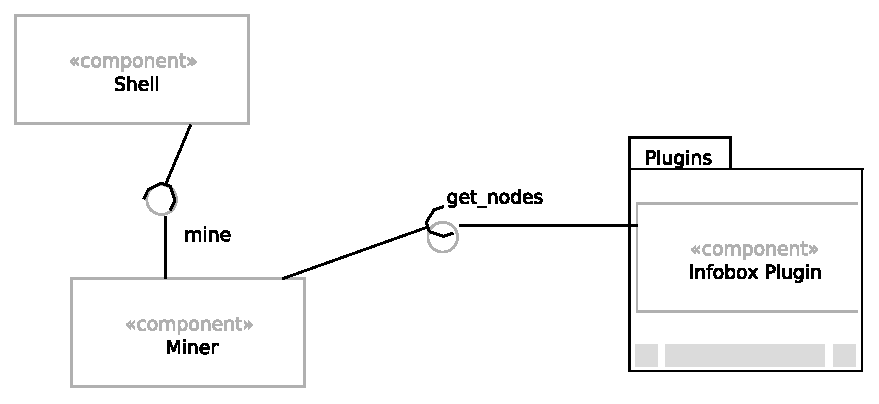
\includegraphics[width=12cm]{ArtistGraph_Architecture.PDF}
\caption{Component Diagram of the ArtistGraph model}
\label{componentdiagram}
\end{figure*}

In order for our application to scale easily if needed, a coding framework needed to be selected. This project 
requires a framework that would be easily extensible to parallel computing at a later phase of 
coding while also allowing us to develop portions locally. Initially, Hadoop seemed like 
a viable option, as it is a popular solution for large parallel applications. However, 
this choice would not allow us to execute different pieces of code simultaneously. Because 
Hadoop requires a single algorithm for each reduction step, it was not our choice for this project. 

Our eventual choice of framework for the implementation of our application was PyMW \cite {ieee5161132}. 
This was chosen because it will allow for a ``Generic Interface'' to be used for development. 
This interface can then be transparently switched to a MPI interface for parallel computing and 
benchmarking. It is important to notice that the original code samples for PyMW fell short from
providing information on how to invoke object methods remotely (as opposed to invoking functions
that are part of the standard Python distribution) but these challenges were overcome by
understanding the way this framework splits code for remote execution and applying knowledge
of Python's implementation of Object Oriented Programming: since the framework will call a method and pass parameters
specified by the user, we specify a bound method and pass the \emph{self} parameter from the code in the master. This
takes advantage of the fact that Python's bound method are treated the same as unbound methods. Furthermore, the lack of
Object Oriented support in the framework was evident by the fact that the intermediate scripts generated from the
interface were named after the method being called. While this seems to be a sensible design decision in principle, it
causes collisions when the same method (in our case, named {\tt get\_nodes}) is called on different objects through the
framework. To overcome this design limitation, the original code of the PyMW framework was patched to use a \emph{fully
  qualified} method name that  includes the module and the class to which the method belongs. This was done in a way
that is backwards compatible to the way unbound methods were named originally.

One significant property of the way PyMW handles the submissions of tasks, even in the simplified ``Generic Interface'',
is that code is effectively copied over to a different file. This is important because references to file positions as
found in the original code are not preserved. This property means debugging strategies like breakpoints cannot be used
in the regular, which complicates the already difficult task of debugging parallel code.

\section{Database Design}
\label{db design}

The first step in designing the schema for our artist database was deciding what data would be important
for us to meet the goals of our project. Any information that could be used to connect one music artist 
to another was determined to be important. This included the albums they created, which labels they were 
under over their career, any tours and performances they participated in, where they were from, and what 
genres of music they produce. All of this information can be used to create connections between artists for 
the user, so that they can explore new music similar to what they currently enjoy.

Once the important data elements were determined, we were able to create a schema for a database that would 
allow us to store the data that we mined about each artist. At the center of the schema is the ARTIST entity, 
which contains the stage name, real name, ID, and origin (city, state, country) of the artist. Branching out 
from the ARTIST entity are a variety of associative entities including: ARTIST-GENRE, TOUR-ARTIST, ASSOC-ARTIST, 
and ALBUM-ARTIST. These entities hold the primary keys from both the ARTIST entity and the other entity that 
they are associated with. For example, TOUR-ARTIST contains both artistID and tourID. This helped us resolve 
the many-to-many relationships that occurred between the entities. In the TOUR entity, the ID and the name of 
the tour are stored. Since a tour can have many performances, we also stored the date, venue, and id of the 
performance in the PERFORMANCE entity.

The GENRE entity contains the id and the genre name so we can draw connections between artists based on their 
genre(s). The ALBUM entity contains information about the albums that an artist has produced. This includes the 
ID, title, release date, number of tracks, number of units sold, and the ID of the label it was produced under 
if it was produced under a label. This label ID references the attribute by the same name in the LABEL entity, 
which contains the label name, the founder, and the date it was founded. If an artist is independent, they will 
not have a label. If that is the case, they can be assigned the label ID that corresponds to a record in the 
LABEL entity that has "Independent" as the label name and nulls for the other fields.

Last, but not least, there is the ASSOC-ARTIST entity. This creates an explicit connection between one artist 
and another. This is accomplished by having both parts of the primary key refer to the artist ID in the ARTIST 
entity. Since an artist may be associated with many artists, it was necessary to create a separate table instead 
of having a multi-valued attribute in the ARTIST entity.

\begin{figure}[hbtp]
\centering
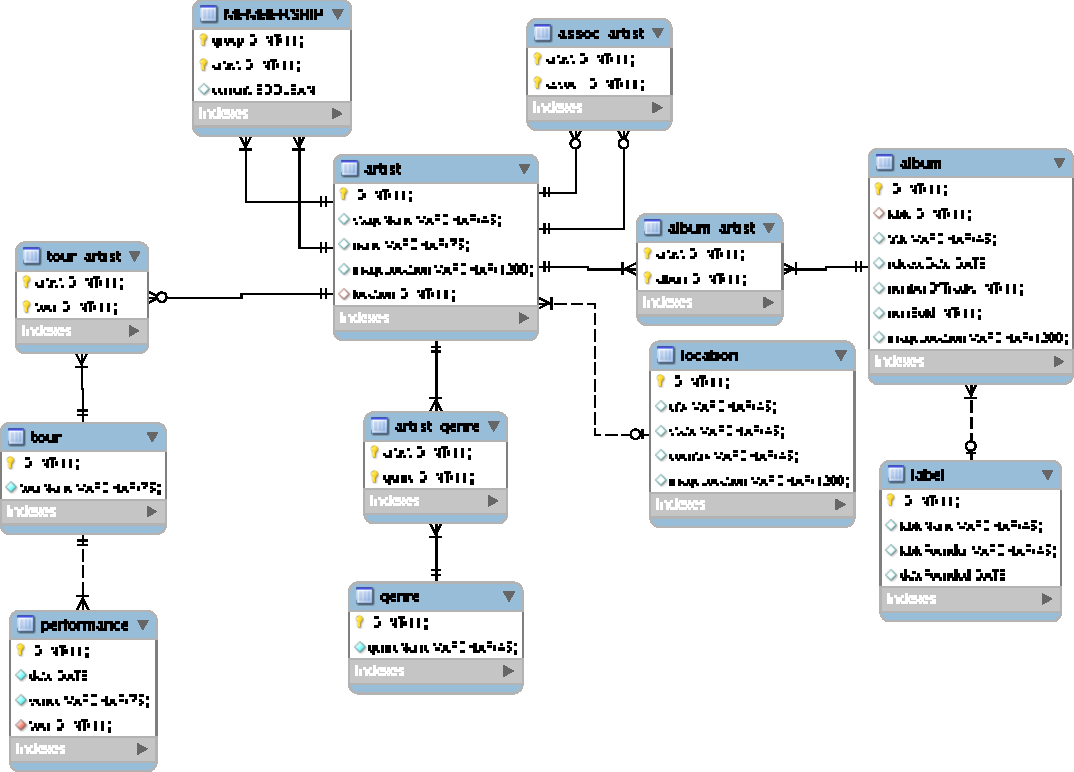
\includegraphics[width=8cm]{ArtistDB.pdf}
\caption{A diagram of the Database Design}
\label{ArtistDB}
\end{figure}

\section{UI Design}
\label{ui design}

The user interface (UI) for the application needed to be developed in two steps. First, the physical appearance 
and layout of the interface, followed by the coding associated with creating the actual interface. Both of these 
tasks are important in providing the user with a simple and enjoyable experience using the application, while 
still connecting the user with the information in our database. 

For the first portion of the design, a basic drawing was created to imitate the final design. The basic premise 
of the interface is a series of connected nodes. Each node will represent an artist, group, or other wikipedia 
page. The initial node will need to be searched using a standard search bar which can be accessed at any time 
the application is being used. Once an artist is searched, his node will appear in the center of the display 
with all of his related nodes displayed around the outside of the central node and connected by line segments. 
Each node will be a basic rectangular shape with tapered edges and display the artists name in or around the node. 
From this central node, the user can choose any surrounding node to become the next central node. This can continue 
as the user desires to map the connection from the original artist to any other artist who is connect through nodes.
Another function of the application that may make it into the final design is a "degrees of separation" counter. 
This would count each time the user chose a node that was connected to the current central node. 

The design was then implemented using QML, a language for rapid development of interactive user interfaces that is part
of the Qt Project. Another project named PyQt4 provides Python bindings that enable easy integration of the QML layout
with our code. The integration of a user interface with the mining code requires a multithreaded message passing system
to be able to present results and interact with the user while mining new nodes in the background.

\section{Lessons Learned}
\label{mistakes}

Scientific code is often regarded as code that delivers good results at the cost of poor quality when compared to
software targeted to wider audiences. Scientific code usually has been tailored and tested to provide accurate, high
performance results; but skips some basic Software Engineering principles and stages in the creation process. This has
been subject of many studies \cite{Li:2011:RSS:1985782.1985789,Phadke:2005:PRM:1145319.1145337} and it is important to
note that there are many projects providing scientific code that cannot be framed into this description. Yet, our
experience with PyMW, as detailed in section \ref{architecture and code}, was that we found a terse documentation and
needed to spend a significant amount of time reading the source code to understand and accomodate our use case to the
expectations of the framework. On the other hand, the fact that the code is Free Software made it possible for us to
modify the sources to accomodate it to our needs. Once all of these changes were in place, we were able to contact Eric
Heien of Computational Infrastructure for Geodynamics, University of California, Davis, the original author of PyMW, to
incorporate these changes in the next release. This is an example of how Free Software in research allows for a more
dynamic development and collaboration.

\section{Current Status and Future Work}
\label{current status}

At the moment, the Database Design covers more concepts and properties than what the code provides. One of the short
term goals is to match the code implementation with the Database Design. After this goal is achieved, we can further
expand the set of entities and properties mined from the data.

Section \ref{ui design} also mentions some of the ideas for the User Interface that need to be implemented. The first
step in this process will be deciding on a good visual toolkit to build upon. This initial design will then be
iteratively tested against the different versions of the Database Design as it is upgraded.

\bibliographystyle{abbrv}
\bibliography{termpaper}
\balance
\end{document}
